\documentclass[12pt]{article}
\usepackage[a4paper,margin=0.75in]{geometry}
\usepackage[utf8]{inputenc}
\usepackage[OT1]{fontenc}
\usepackage[table,usenames,dvipsnames]{xcolor}
\usepackage{array}
\usepackage{varwidth}
\usepackage{multirow,tabularx}
\usepackage{amsmath}
\usepackage{hyperref}
\usepackage{enumitem}
\usepackage{physics}
\usepackage{graphicx}
\usepackage{tcolorbox}
\renewcommand*\familydefault{\sfdefault}

\newtcolorbox{mybox}[3][]
{
  colframe = #2!25,
  colback  = #2!10,
  coltitle = #2!20!black,  
  title    = {#3},
  #1,
}

\hypersetup{
    colorlinks=true,
    linkcolor=blue,
    filecolor=magenta,      
    urlcolor=cyan,
    pdftitle={Overleaf Example},
    pdfpagemode=FullScreen,
}

\title{\textbf{COL774 Assignment 3}}
\author{Aniruddha Deb \\ \texttt{2020CS10869}}
\date{October 2022}

\begin{document}

\maketitle

\section{Decision Trees, Random Forests, Gradient Boosted Trees}

\subsection{Dataset 1}

\begin{enumerate}[label=(\alph*)]
    \item After removing the missing values, we obtain the following accuracies:
    \begin{enumerate}[label=(\roman*)]
        \item \textbf{Training set:} 92.53 \%
        \item \textbf{Validation set:} 76.03 \%
        \item \textbf{Test set:} 69.17 \%
    \end{enumerate}

    The decision tree we obtain is as follows (drawn upto a depth of 3):
    \begin{center}
        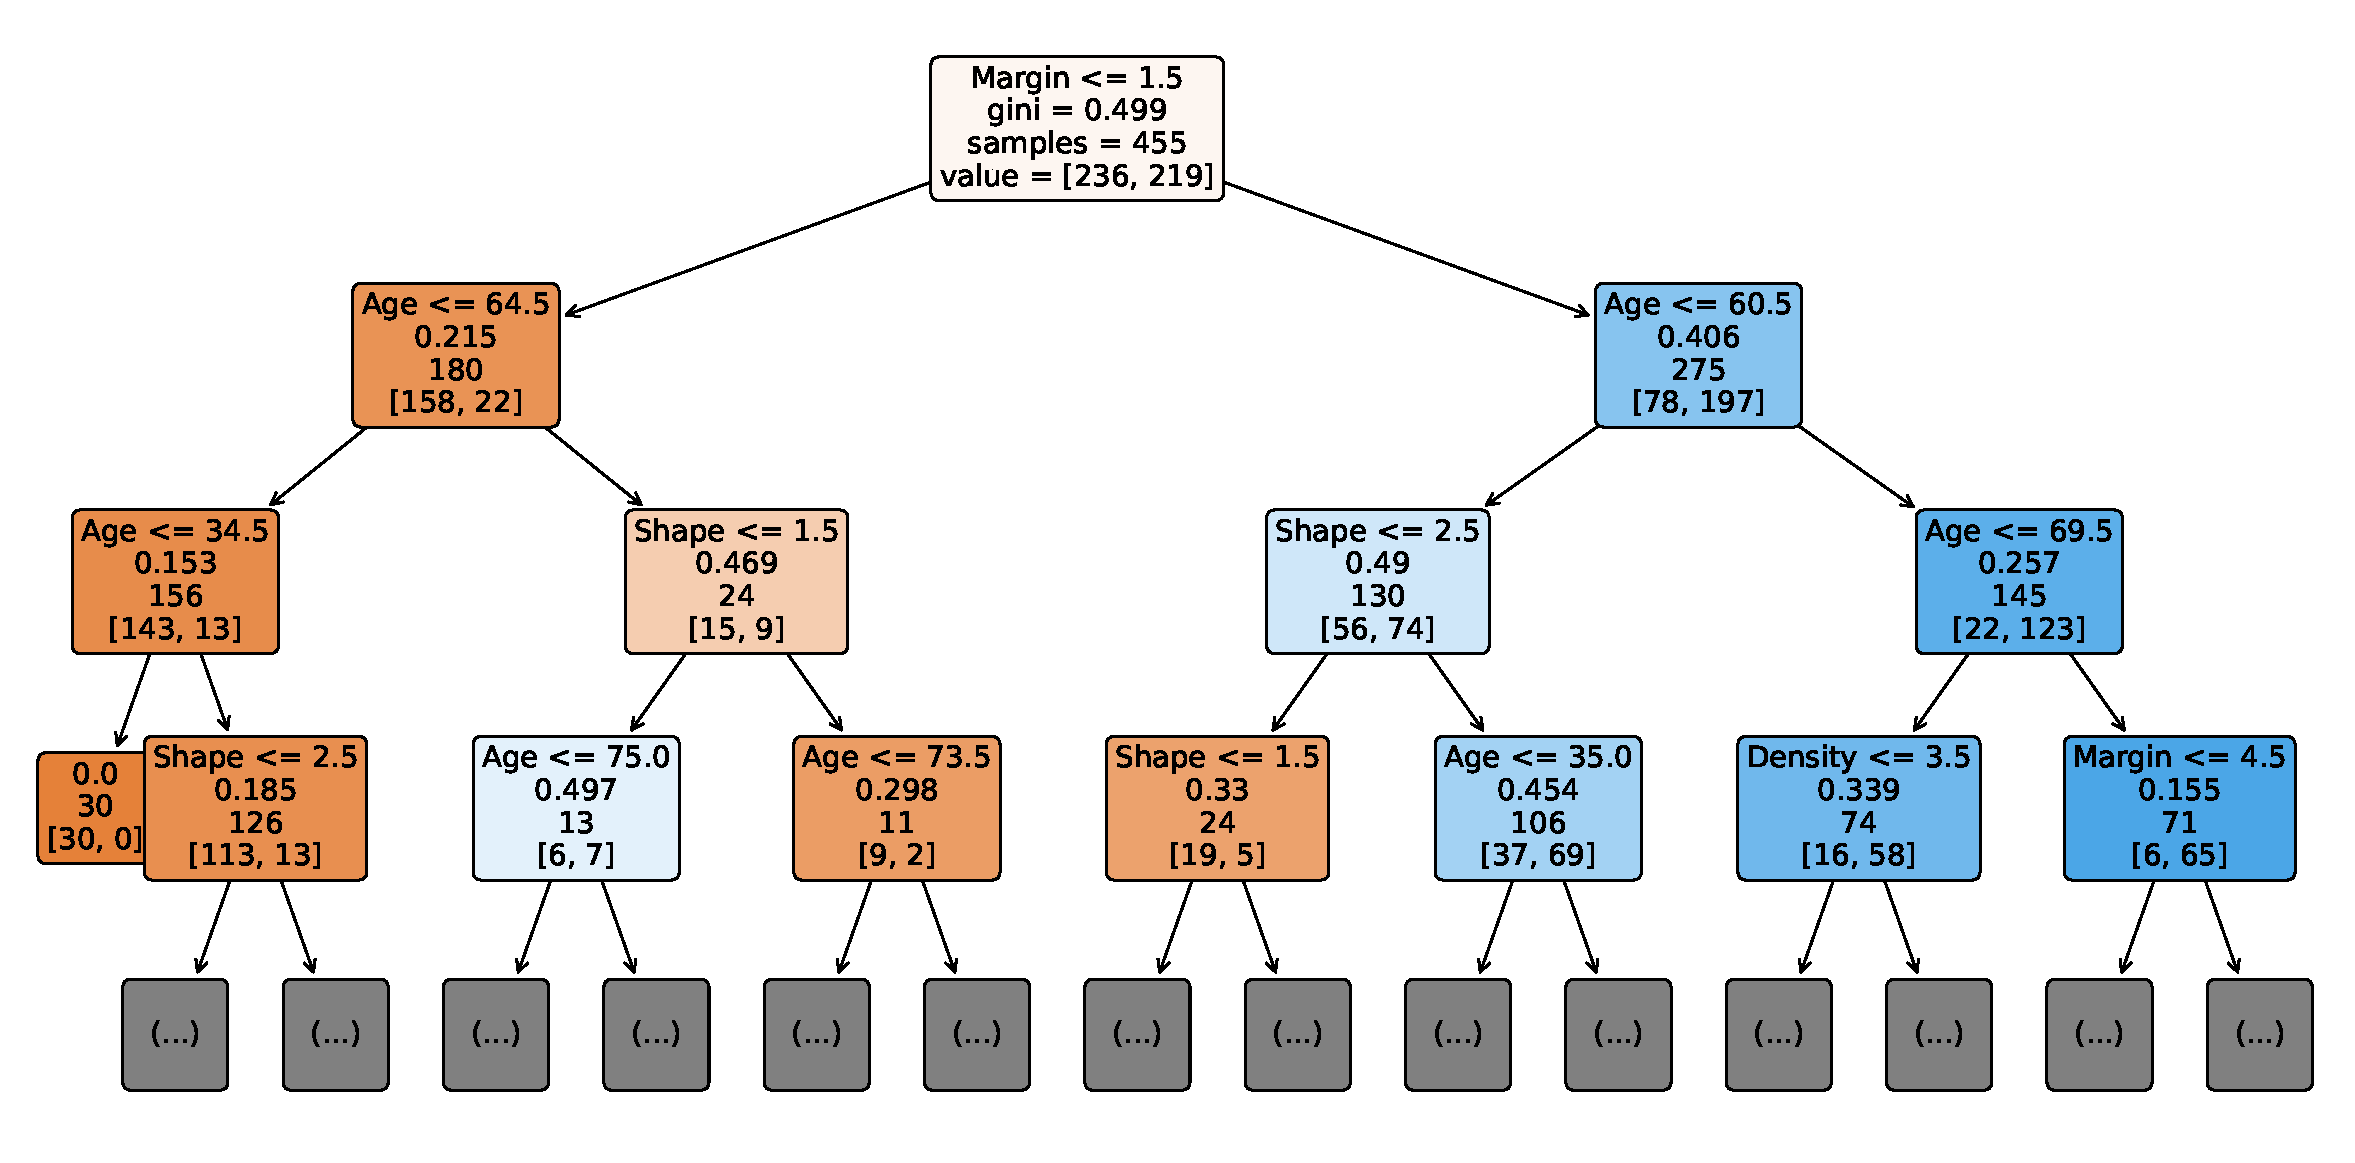
\includegraphics[width=0.94\textwidth]{../Q1/tree.pdf}
    \end{center}

    \item With GridSearchCV and the grid of parameters $\text{max\_depth}=\{4,6,8,10\}$, 
    $\text{min\_samples\_split}=\{2,3,4,5\}$ and $\text{min\_samples\_leaf}=\{1,2,3,4,5\}$,
    the best parameters (obtained via five-fold cross validation) are:
    \begin{enumerate}[label=(\roman*)]
        \item max\_depth = 4
        \item min\_samples\_leaf = 5
        \item min\_samples\_split = 2
    \end{enumerate}

    With them, we obtain the following accuracies:
    \begin{enumerate}[label=(\roman*)]
        \item \textbf{Training set:} 81.98 \%
        \item \textbf{Validation set:} 87.6 \%
        \item \textbf{Test set:} 75.1 \%
    \end{enumerate}

    The decision tree has a much shallower depth than the previous tree, and is
    also simpler

    \begin{center}
        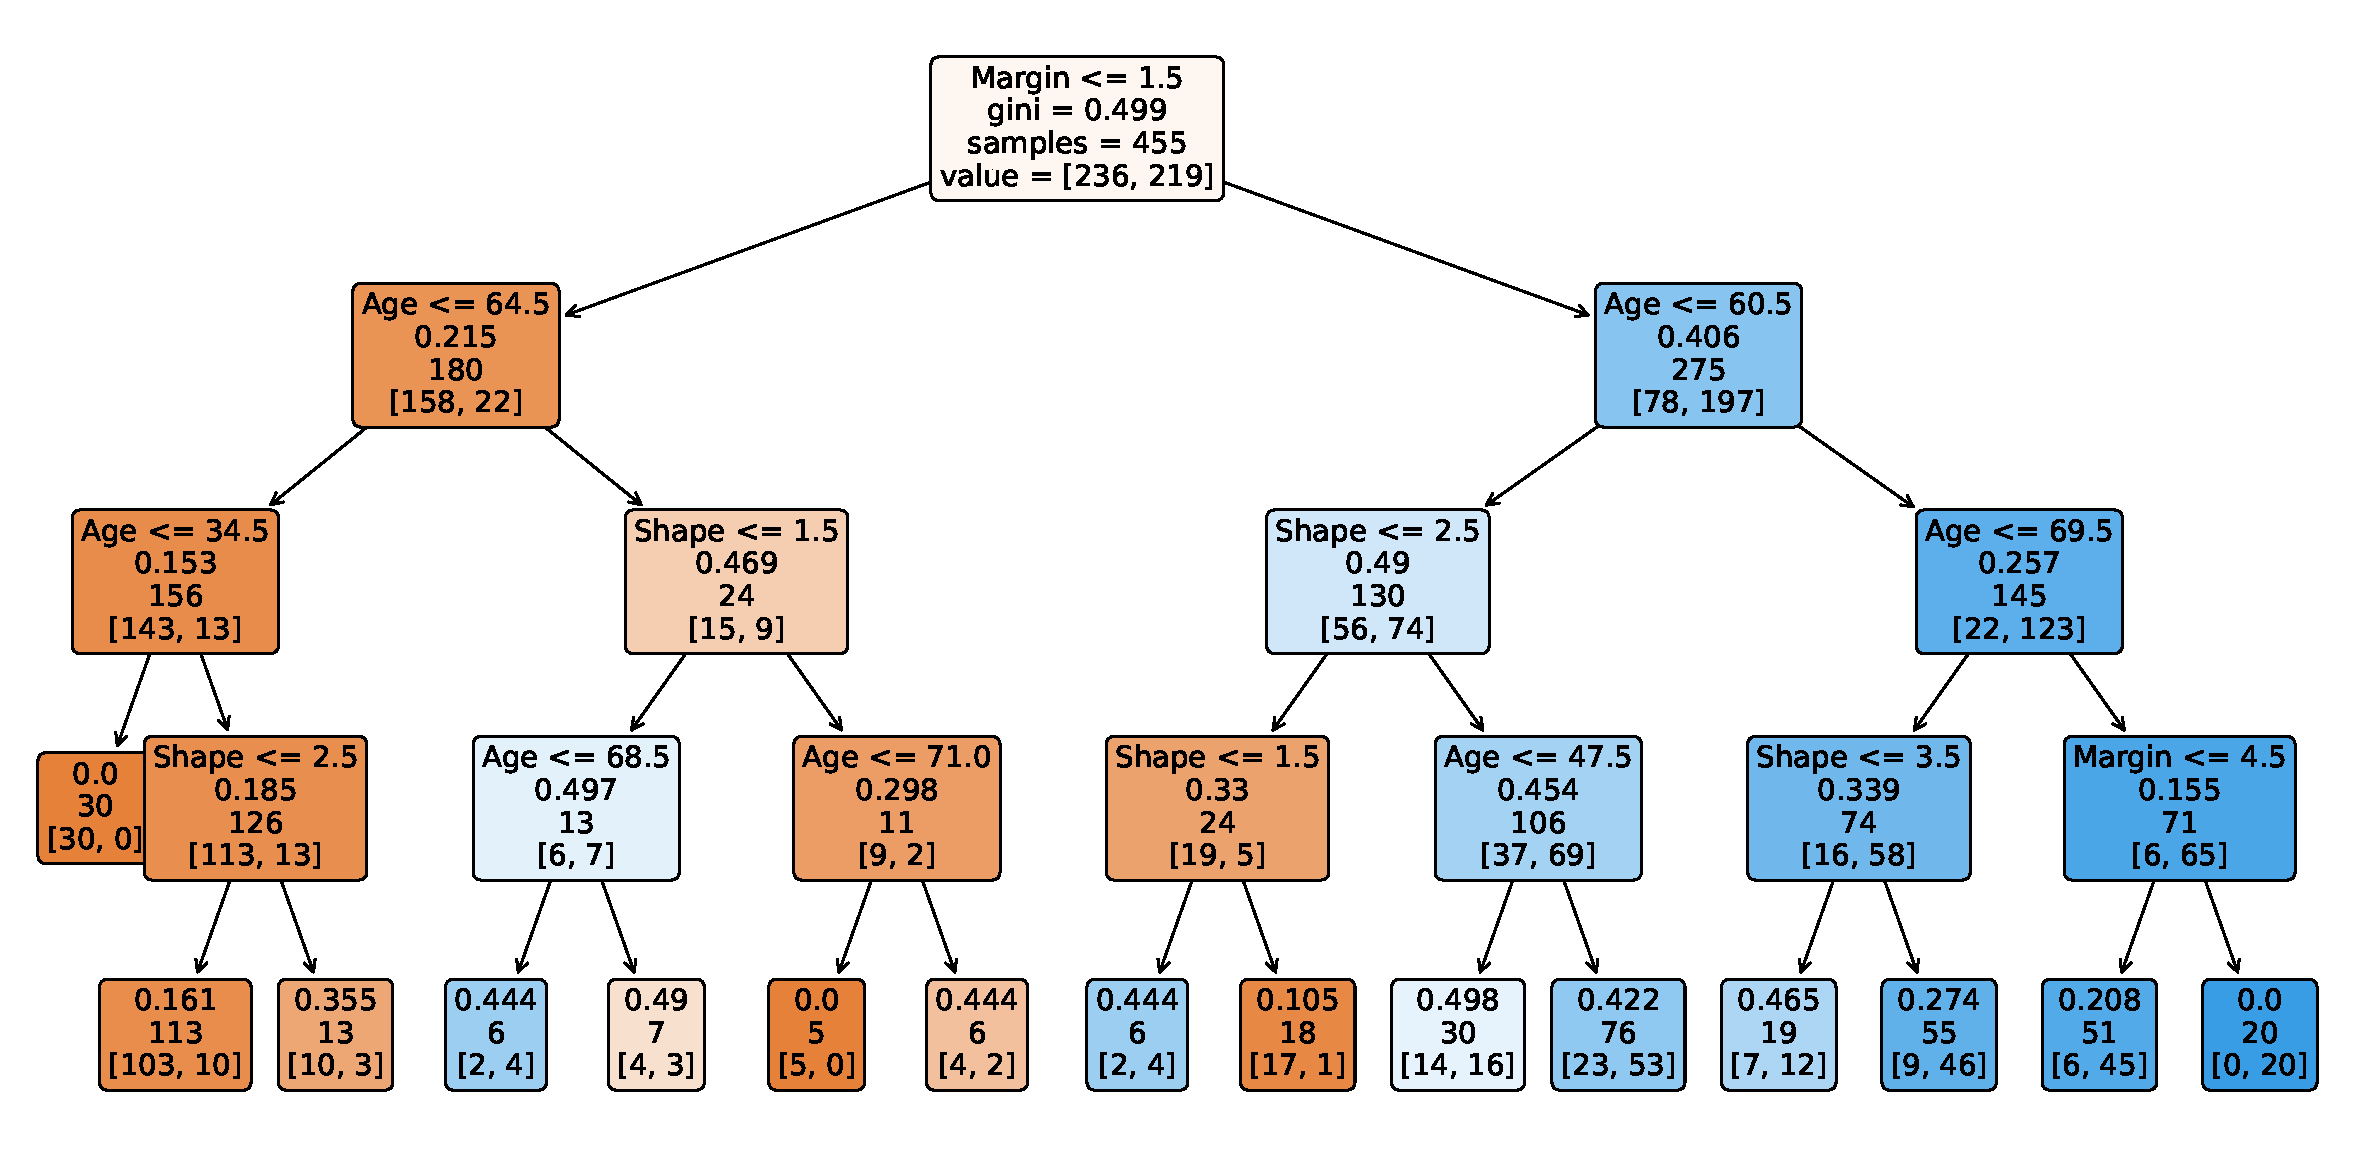
\includegraphics[width=0.94\textwidth]{../Q1/tree_optimal.pdf}
    \end{center}

    \item The total impurity vs the alphas is plotted below, along with the depth
        and the number of nodes v/s alpha

    \begin{center}
        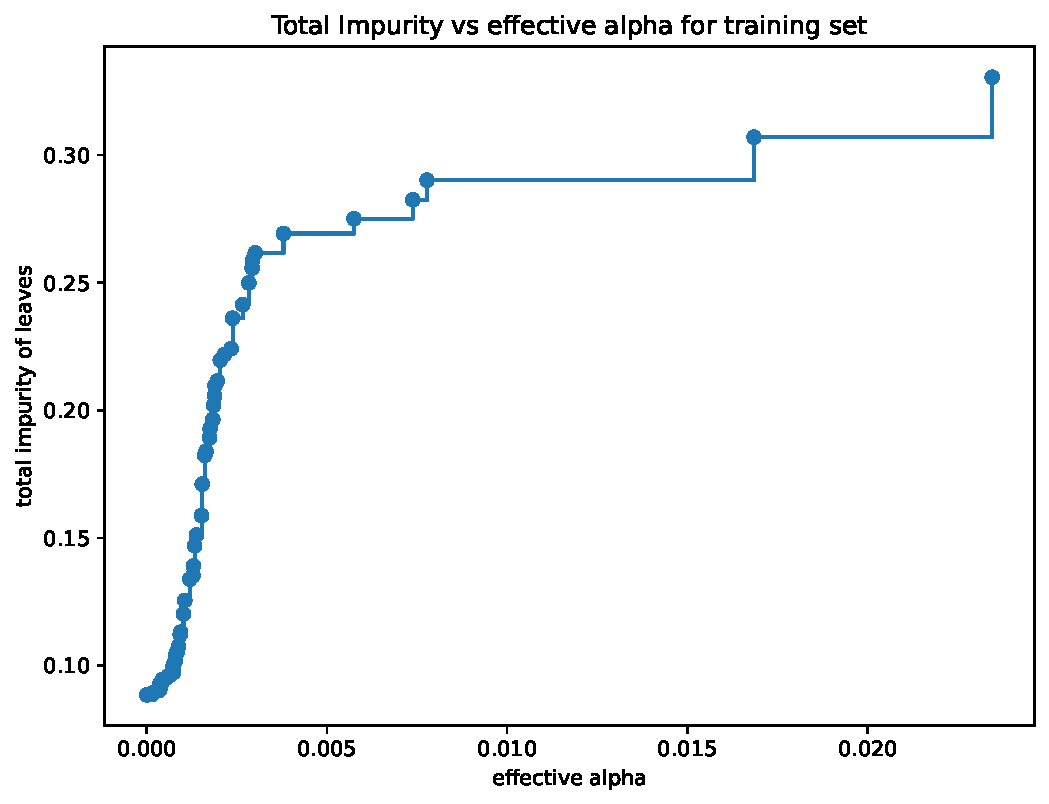
\includegraphics[width=0.45\textwidth]{../Q1/impurity_vs_alpha.pdf}
        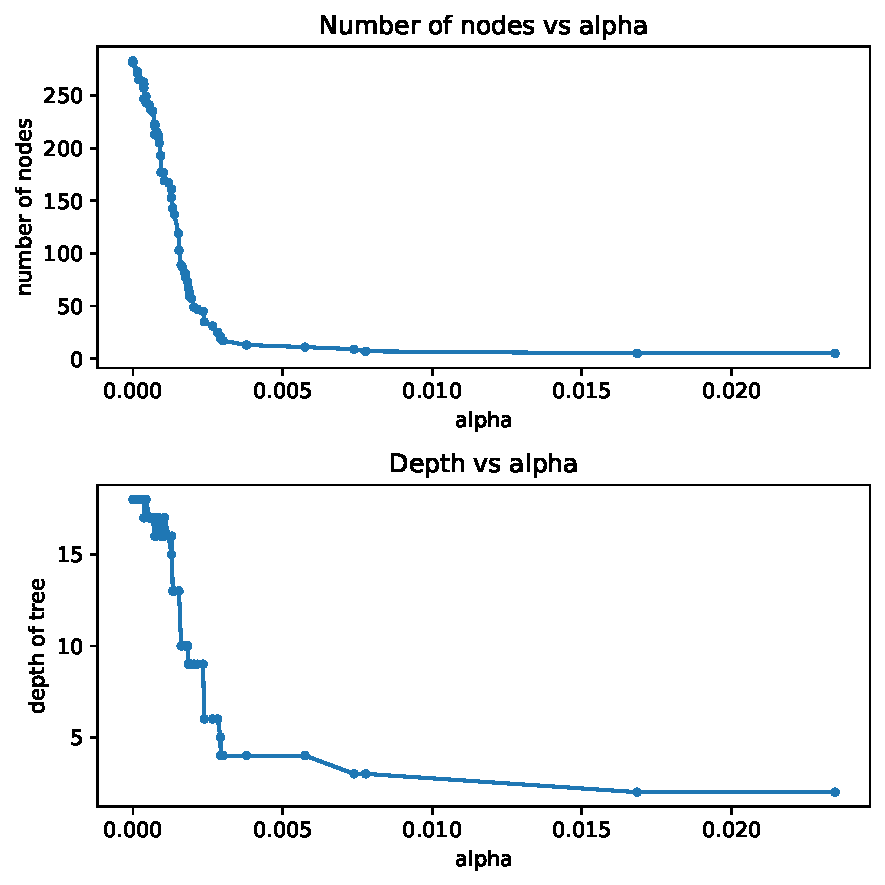
\includegraphics[width=0.45\textwidth]{../Q1/nodes_vs_alpha.pdf}
    \end{center}

    We see that the training accuracy is very high for low values of alpha, at 
    the expense of the validation and test accuracy i.e. the model overfits for 
    low values of alpha. The best trees are the ones with fewer nodes

    \begin{center}
        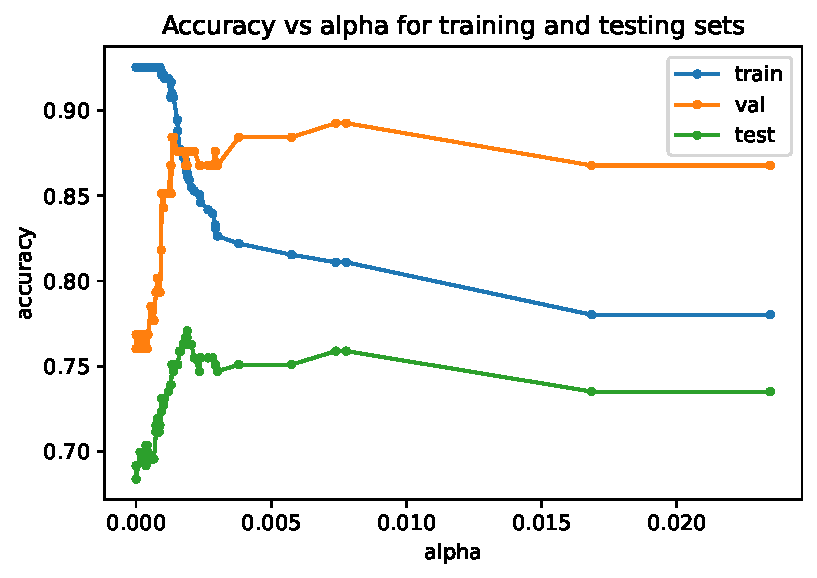
\includegraphics[width=0.6\textwidth]{../Q1/accuracy_vs_alpha.pdf}
    \end{center}

    The accuracies we obtain for the various datasets, using the best pruned tree
    are:
    \begin{enumerate}
        \item \textbf{Training set:} 81.1 \%
        \item \textbf{Validation set:} 89.26 \%
        \item \textbf{Test set:} 75.89 \%
    \end{enumerate}

    The best pruned tree, as discussed before, has only 9 nodes compared to the 
    trees we obtained in part (a) and part (b). 

    \begin{center}
        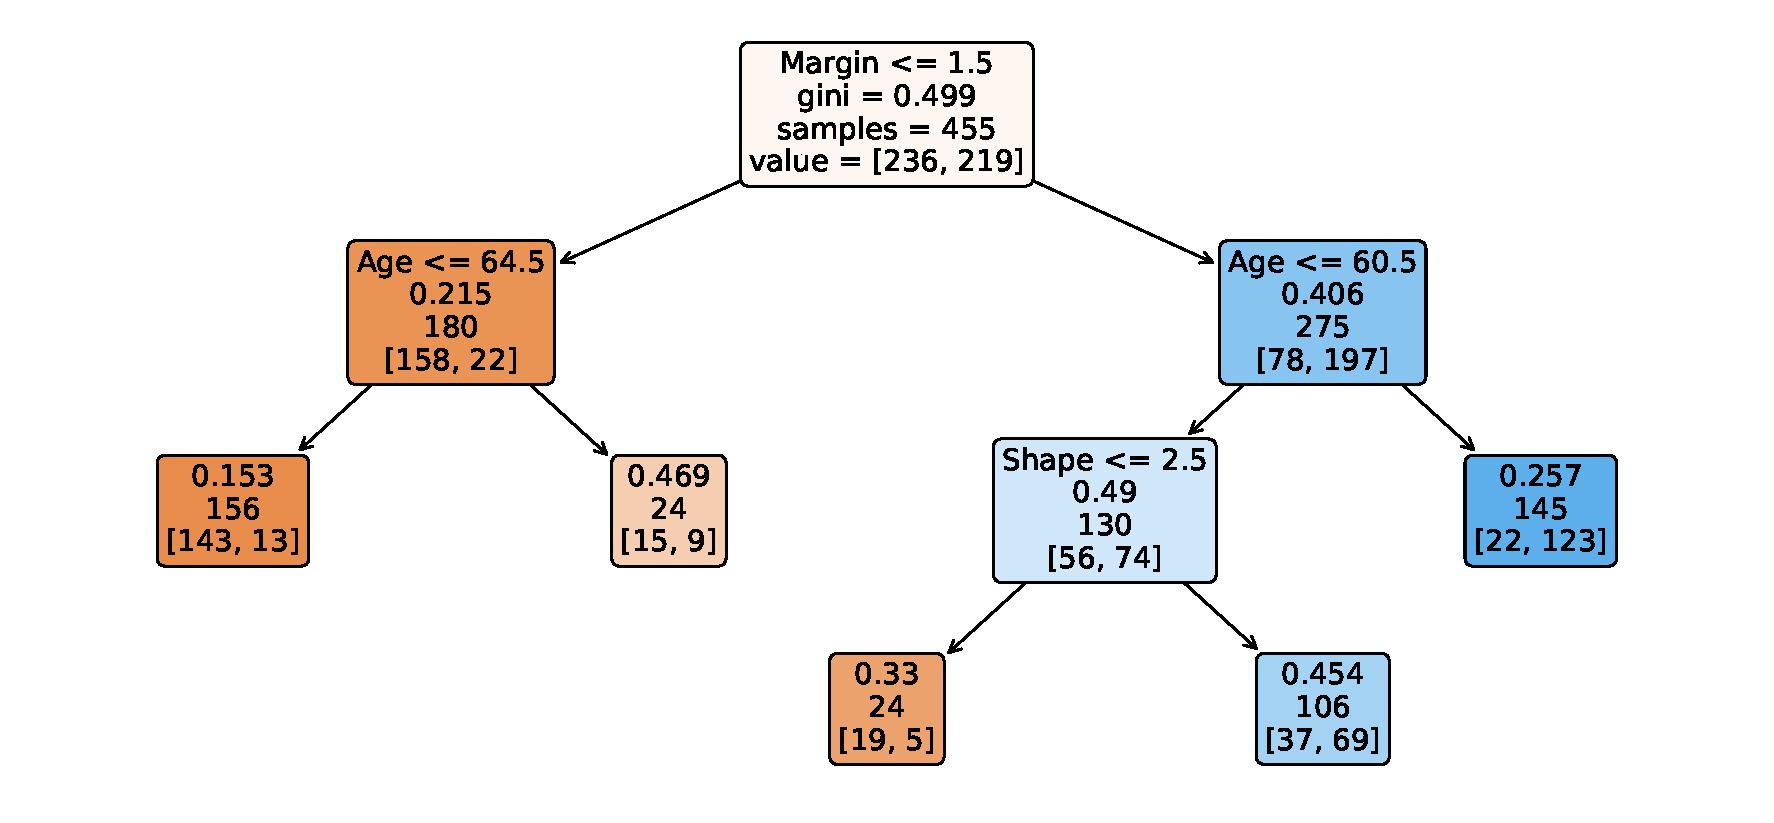
\includegraphics[width=0.94\textwidth]{../Q1/tree_best_pruned.pdf}
    \end{center}

    \item With GridSearchCV and the grid of parameters $\text{n\_estimators}=\{50, 100, 150, 200\}$, \\
    $\text{max\_features}=\{1,2,3,4\}$ and $\text{min\_samples\_split}=\{2,3,4,5\}$,
    the best parameters (obtained using out of bag score as the metric) are:
    \begin{enumerate}[label=(\roman*)]
        \item n\_estimators = 200
        \item min\_samples\_split = 5
        \item max\_features = 3
    \end{enumerate}

    With them, we obtain the following accuracies:
    \begin{enumerate}[label=(\roman*)]
        \item \textbf{Training set:} 90.11 \%
        \item \textbf{Out of Bag set:} 76.26 \%
        \item \textbf{Validation set:} 86.78 \%
        \item \textbf{Test set:} 76.68 \%
    \end{enumerate}

    \item The results are summarized in the following table:

    \begin{center}
    \begin{tabular}{l c c}
        Default decision tree: & Median & Mode \\
        \hline
        \hspace{3mm} Train & 91.81 \% & 90.69 \% \\
        \hspace{3mm} Validation & 74.07 \% & 75.56 \% \\
        \hspace{3mm} Test & 74.31 \% & 71.18 \% \\
             & & \\
        Grid Searched Decision tree: & Median & Mode \\
        \hline
        \hspace{3mm} max\_depth & 4 & 4 \\
        \hspace{3mm} min\_samples\_split \hspace{30mm} & 2 & 2 \\ % hack for some space
        \hspace{3mm} min\_samples\_leaf & 3 & 2 \\
        \hspace{3mm} Train & 81.56 \% & 81.38 \% \\
        \hspace{3mm} Validation & 87.41 \% & 86.67 \% \\
        \hspace{3mm} Test & 80.90 \% & 77.43 \% \\
            & & \\
        ccp\_alpha optimized Decision tree: & Median & Mode \\
        \hline
        \hspace{3mm} n\_nodes & 11 & 137 \\
        \hspace{3mm} ccp\_alpha & 0.0055 & 0.0012 \\
        \hspace{3mm} Train & 80.26 \% & 88.83 \% \\
        \hspace{3mm} Validation & 87.41 \% & 88.15 \% \\
        \hspace{3mm} Test & 79.17 \% & 76.04 \% \\
            & & \\
        Random Forest classifier: & Median & Mode \\
        \hline
        \hspace{3mm} n\_estimators & 200 & 100 \\
        \hspace{3mm} min\_samples\_split & 5 & 5 \\
        \hspace{3mm} max\_features & 3 & 2 \\
        \hspace{3mm} Train & 88.45 \% & 88.08 \% \\
        \hspace{3mm} Out of Bag & 75.23 \% & 73.37 \% \\
        \hspace{3mm} Validation & 83.70 \% & 83.70 \% \\
        \hspace{3mm} Test & 77.78 \% & 77.43 \% \\
    \end{tabular}
    \end{center}

    The imputed tree is marginally better (2-3 \%) compared to the tree which 
    ignores missing values. Note that the comparision is not exact, as the size 
    of the validation and test sets are also changing as a consequence (while 
    ignoring missing values, we also ignore the ones in the test and validation 
    set). As a result, the actual increase in accuracy post imputation will be 
    much more than that without imputation.
    
    \item After implementing an XGBoost classifier and searching for parameters
    using GridSearchCV in the given parameter space, we obtain the following 
    best parameters:
    \begin{enumerate}[label=(\roman*)]
        \item max\_depth = 10
        \item n\_estimators = 10
        \item subsample = 0.5
    \end{enumerate}

    With them, we obtain the following accuracies:
    \begin{enumerate}[label=(\roman*)]
        \item \textbf{Training set:} 83.61 \%
        \item \textbf{Validation set:} 84.44 \%
        \item \textbf{Test set:} 77.08 \%
    \end{enumerate}
\end{enumerate}

\subsection{Dataset 2}

NOTE: This dataset was not completely evaluated due to the large running time 
of grid search on the dataset

\begin{enumerate}[label=(\alph*)]
    \item Fitting a decision tree on the entire dataset gave us the following 
        accuracies:
    \begin{enumerate}[label=(\roman*)]
        \item \textbf{Training set:} 100 \%
        \item \textbf{Validation set:} 58.49 \%
        \item \textbf{Test set:} 57.74 \%
    \end{enumerate}

    \item Grid search was run on the following parameter space:
    \begin{enumerate}[label=(\roman*)]
        \item \texttt{max\_depth}: $\{10, 15, 20, 25, 30\}$
        \item \texttt{min\_samples\_split}: $\{2,3,4\}$
        \item \texttt{min\_samples\_leaf}: $\{1,2,3\}$
    \end{enumerate}

    The best parameters were:
    \begin{enumerate}[label=(\roman*)]
        \item \texttt{max\_depth}: 30
        \item \texttt{min\_samples\_split}: 2
        \item \texttt{min\_samples\_leaf}: 1
    \end{enumerate}

    The accuracies for these parameters are:
    \begin{enumerate}[label=(\roman*)]
        \item \textbf{Training set:} 63.17 \%
        \item \textbf{Validation set:} 44.30 \%
        \item \textbf{Test set:} 44.01 \%
    \end{enumerate}

\end{enumerate}

The kernel timed out after this point, which is why no more statistics were 
obtained.

\pagebreak

\section{Neural Network}

\begin{enumerate}[label=(\alph*)]
    \item The neural network was implemented in Numpy, in a purely functional 
    manner (so it can support any activation, loss and learning rate function 
    passed to it). Forward propagation is given by the following equations:
    \begin{align*}
        z_i &= l_{i-1} \times w_i + b_i \\
        l_i &= \text{act}(z_i)
    \end{align*}
    where $l_i$ is the output of the $i$th layer, $z_i$ is the linear output 
    of the perceptrons and $\text{act}$ is the activation function. Note that we 
    use $\times$ to denote matrix multiplication and $\odot$ to denote Hadamard
    (elementwise) multiplication.

    Backward propagation is given by the following equations:
    \begin{align*}
        \pdv{J}{l_L} &= \text{loss'}(\theta) \\
        \\
        \pdv{J}{w_i} &= \pdv{J}{l_i} \pdv{l_i}{z_i} \pdv{z_i}{w_i} \\
                     &= l_{i-1}^T \times \left( \pdv{J}{l_i} \odot \text{act'}(z_i) \right) \\
        \\
        \pdv{J}{b_i} &= \pdv{J}{l_i} \pdv{l_i}{z_i} \pdv{z_i}{b_i} \\
                     &= \pdv{J}{l_i} \odot \text{act'}(z_i) \\
        \\
        \pdv{J}{l_{i-1}} &= \pdv{J}{l_i} \pdv{l_i}{z_i} \pdv{z_i}{l_i} \\
                     &= \left( \pdv{J}{l_i} \odot \text{act'}(z_i) \right) \times w_i^T 
    \end{align*}

    The matrix initialization was done according to \href{https://arxiv.org/pdf/1502.01852.pdf}{He et al.},
    wherein the matrices $w_i$ and $b_i$ were initialized using a zero-mean 
    normal distribution with variance $\sqrt{2/n_i}$, where $n_l$ is the number 
    of neurons in the $i$th layer.

    \item The network was trained with the stopping criteria that the \% change
    in loss between two consecutive epochs, after training for atleast 50 epochs,
    is less than $10^{-4}$. The network also has an upper bound of 300 epochs 
    for training. 

    The accuracies the trained model obtains on the test dataset, with varying 
    hidden layer sizes, are:
    \begin{center}
        \begin{tabular}{|c|c|c|}
            \hline
            Neurons & Test Accuracy & Train Accuracy\\ 
            \hline 
            5  & 76.1 \% & 77.7 \% \\
            10 & 75.8 \% & 77.1 \% \\
            15 & 80.2 \% & 82.3 \% \\
            20 & 71.9 \% & 73.9 \% \\
            25 & 78.7 \% & 79.9 \% \\
            \hline
        \end{tabular}
    \end{center}

    \begin{center}
        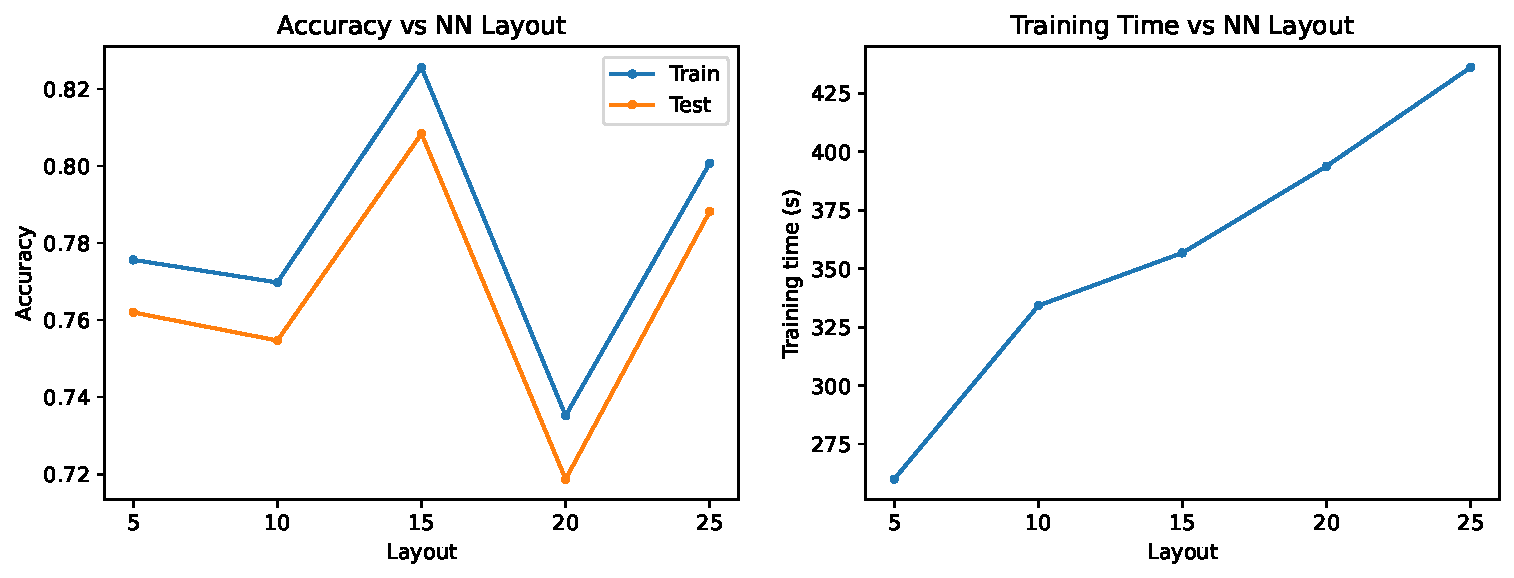
\includegraphics[width=0.9\textwidth]{../Q2/single_layer_sigmoid/acc_time.pdf}
    \end{center}

    The confusion matrices are:
    \begin{center}
        \begin{tabular}{c c c}
            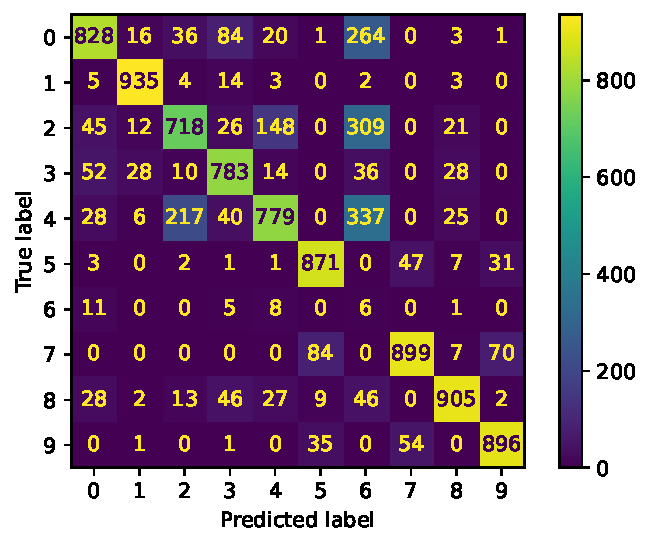
\includegraphics[width=0.27\textwidth]{../Q2/single_layer_sigmoid/cmat_5.pdf} &
            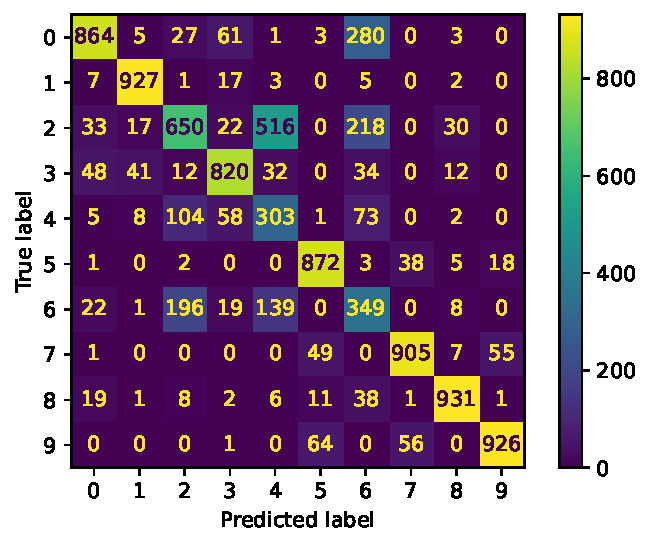
\includegraphics[width=0.27\textwidth]{../Q2/single_layer_sigmoid/cmat_10.pdf} &
            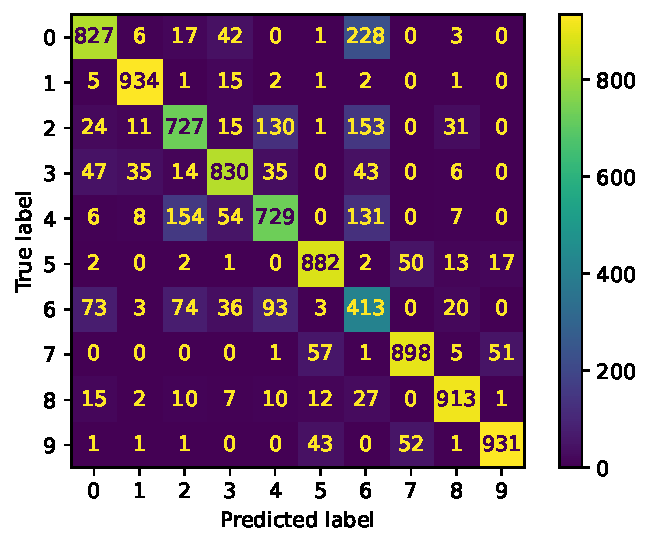
\includegraphics[width=0.27\textwidth]{../Q2/single_layer_sigmoid/cmat_15.pdf} \\
            5 & 10 & 15 
        \end{tabular}

        \begin{tabular}{c c}
            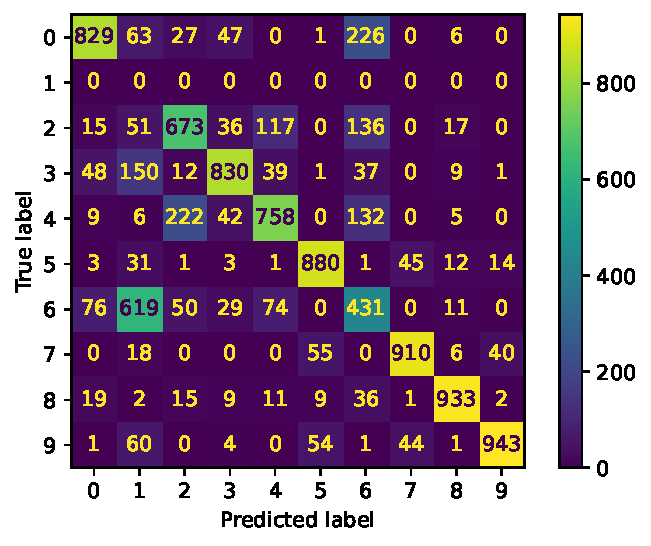
\includegraphics[width=0.27\textwidth]{../Q2/single_layer_sigmoid/cmat_20.pdf} &
            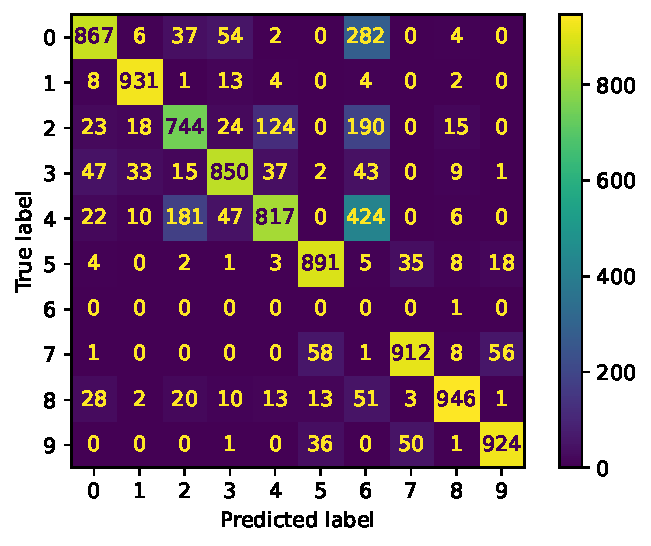
\includegraphics[width=0.27\textwidth]{../Q2/single_layer_sigmoid/cmat_25.pdf} \\
            20 & 25
        \end{tabular}
    \end{center}

    We observe that models with fewer number of neurons tend to marginally 
    underfit, and that there is a dip for models with an even number of neurons 
    in the hidden layer (a zigzag pattern is observed). The training time, 
    as expected, increases with an increase in the number of neurons. 

    Also, note that 20 and 25 may not have completely learnt the model: they 
    do not classify a label correctly (class 1 in the 20-neuron network and class 
    6 in the 25-neuron network). They may give better results if we run the 
    network for a longer period of time with a different convergence criterion.

    \item The stopping condition would now change, as our step size (and consequently
    change in loss) would decrease with increasing epochs. Changing the stopping
    condition to $10^{-4}/\sqrt{e}$, where $e$ is the current epoch, gave the 
    following results:
    \begin{center}
        \begin{tabular}{|c|c|c|}
            \hline
            Neurons & Test Accuracy & Train Accuracy \\ 
            \hline 
            5  & 56.2 \% & 56.4 \% \\
            10 & 71.1 \% & 71.9 \% \\
            15 & 78.5 \% & 79.6 \% \\
            20 & 80.3 \% & 82.3 \% \\
            25 & 80.4 \% & 82.5 \% \\
            \hline
        \end{tabular}
    \end{center}

   \begin{center}
        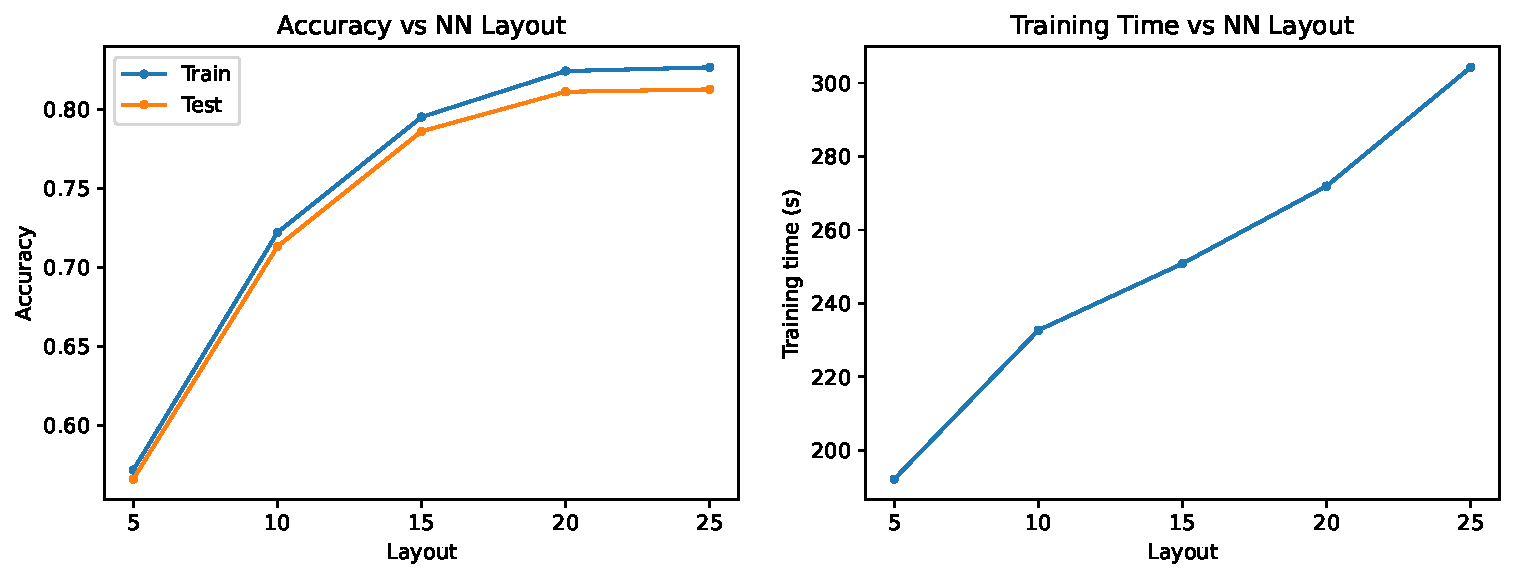
\includegraphics[width=0.9\textwidth]{../Q2/single_layer_sigmoid_epochlr/acc_time.pdf}
    \end{center}

    \begin{center}
        \begin{tabular}{c c c}
            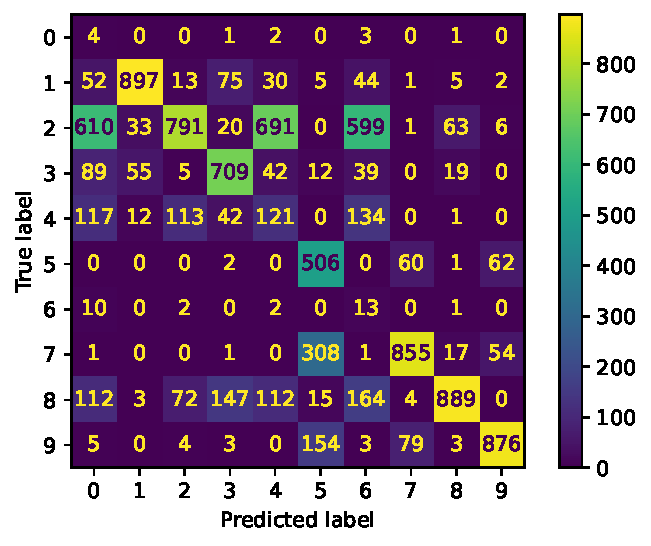
\includegraphics[width=0.27\textwidth]{../Q2/single_layer_sigmoid_epochlr/cmat_5.pdf} &
            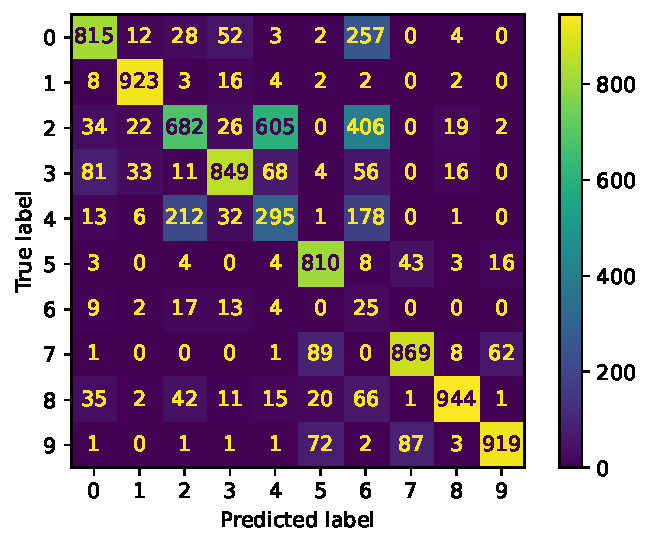
\includegraphics[width=0.27\textwidth]{../Q2/single_layer_sigmoid_epochlr/cmat_10.pdf} &
            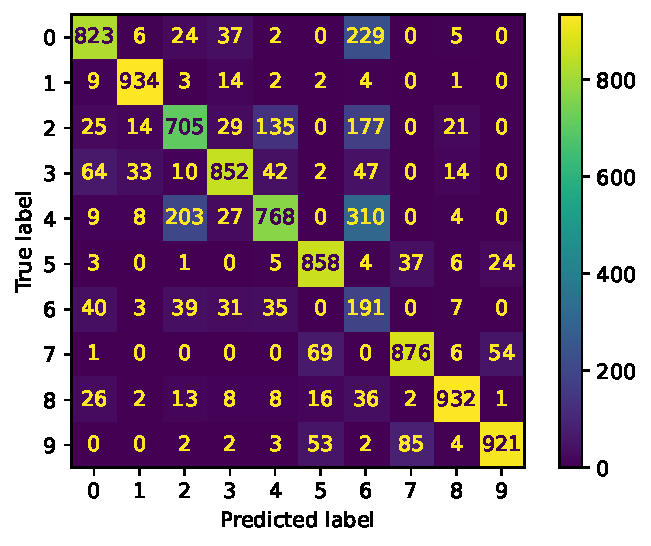
\includegraphics[width=0.27\textwidth]{../Q2/single_layer_sigmoid_epochlr/cmat_15.pdf} \\
            5 & 10 & 15 
        \end{tabular}

        \begin{tabular}{c c}
            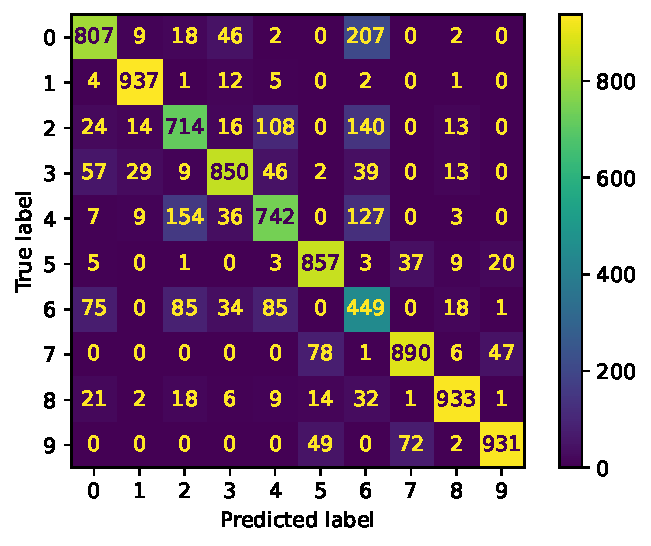
\includegraphics[width=0.27\textwidth]{../Q2/single_layer_sigmoid_epochlr/cmat_20.pdf} &
            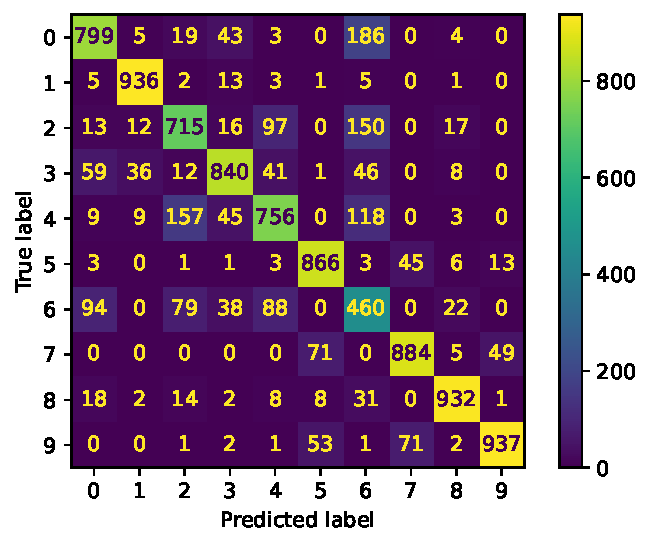
\includegraphics[width=0.27\textwidth]{../Q2/single_layer_sigmoid_epochlr/cmat_25.pdf} \\
            20 & 25
        \end{tabular}
    \end{center}

    The Epoch LR is a slow learner, and in none of the cases above did it converge
    before the epoch limit (200) was hit. In terms of training time, it trained
    faster than the previous network, even though the epoch limit was hit.

    \item With a 2x100 network as described in the assignment, we obtain the 
    following results:

    \begin{center}
        \begin{tabular}{|c|c|c|}
            \hline
            Network & Test Accuracy & Train Accuracy \\ 
            \hline 
            relu    & 78.8 \% & 82.5 \% \\
            sigmoid & 83.4 \% & 85.3 \% \\
            \hline
        \end{tabular}
    \end{center}
    
    \begin{center}
        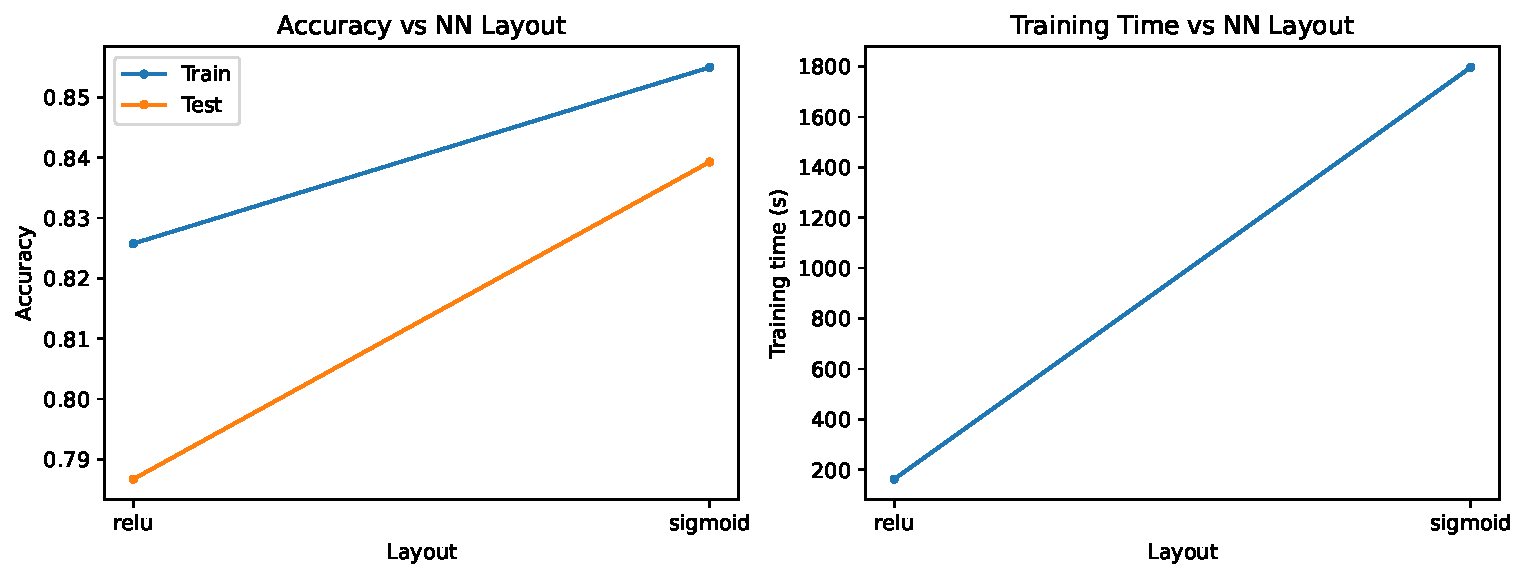
\includegraphics[width=0.9\textwidth]{../Q2/two_layer_relu_sigmoid/acc_time.pdf}
    \end{center}
    \begin{center}
        \begin{tabular}{c c}
            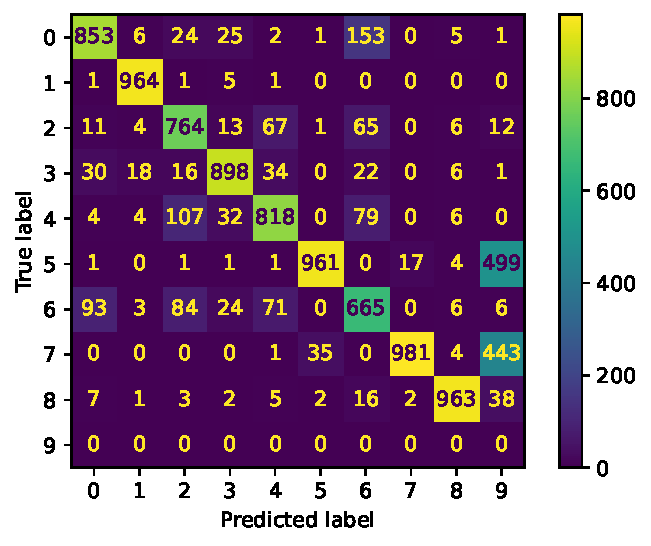
\includegraphics[width=0.4\textwidth]{../Q2/two_layer_relu_sigmoid/cmat_relu.pdf} &
            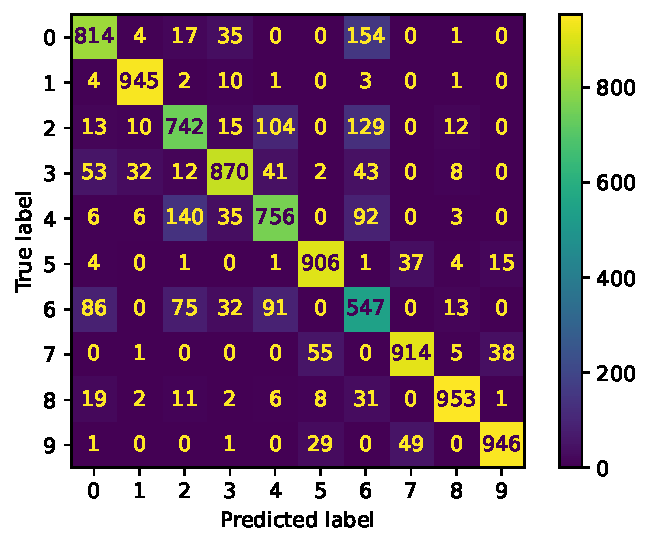
\includegraphics[width=0.4\textwidth]{../Q2/two_layer_relu_sigmoid/cmat_sigmoid.pdf} \\
            relu & sigmoid
        \end{tabular}
    \end{center}

    When both were trained with a fixed number of epochs, the ReLU network performed
    better. This implies that like before, the variable learning rate is not 
    converging to the local minima quickly. The sigmoid performs better as it is
    'easier' to learn than the relu: the derivatives do not go immediately to zero,
    and as a result, the net gradient would be larger than the one obtained from
    ReLU and this would allow it to take larger steps with the adaptive learning 
    rate.

    The results are better than the ones in 2(b): This is to be expected, as more
    neurons allow the network to learn a larger number of hypotheses.

    \item With increasing the number of layers, the accuracy increases until 
    it saturates at 86\% for the test set. The training time graph also indicates
    that the networks with 2 and 3 hidden layers were inadequately trained and 
    hence underfit the data. 

    \begin{center}
        \begin{tabular}{|c|c|c|}
            \hline
            Layers & Test Accuracy & Train Accuracy \\ 
            \hline 
            2 & 73.5 \% & 75.2 \% \\
            3 & 77.2 \% & 82.3 \% \\
            4 & 86.8 \% & 96.1 \% \\
            5 & 86.7 \% & 96.0 \% \\
            \hline
        \end{tabular}
    \end{center}

   \begin{center}
        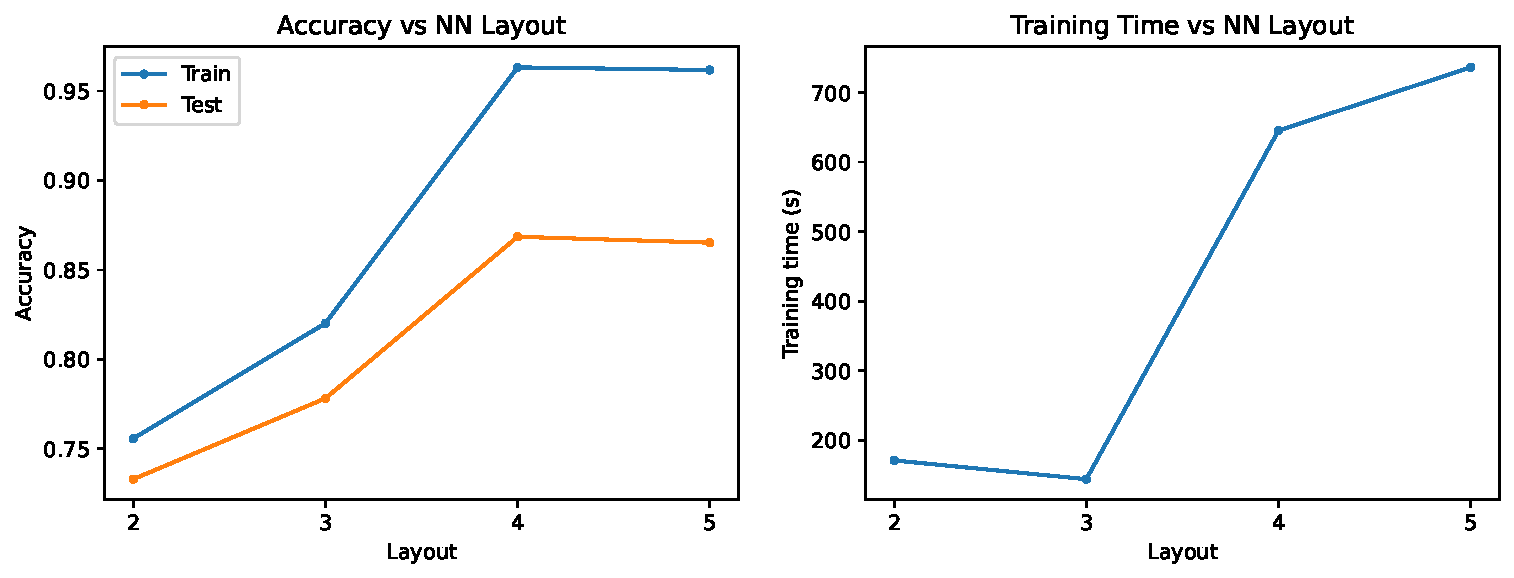
\includegraphics[width=0.9\textwidth]{../Q2/mult_layer_relu/acc_time.pdf}
    \end{center}

    \begin{center}
        \begin{tabular}{c c}
            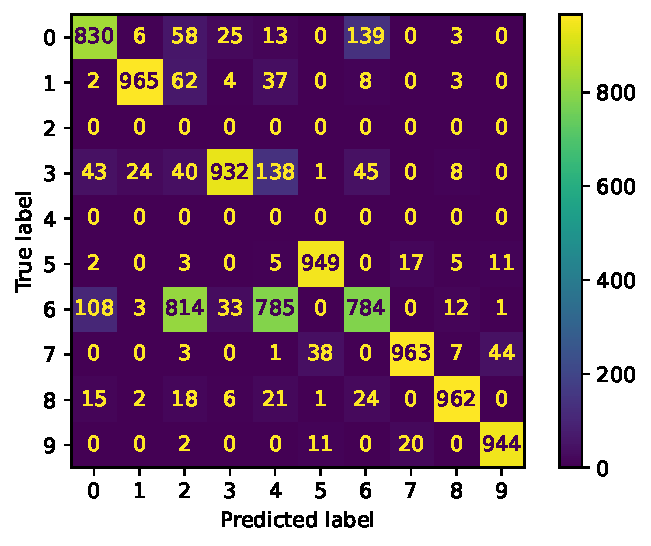
\includegraphics[width=0.35\textwidth]{../Q2/mult_layer_relu/cmat_2.pdf} &
            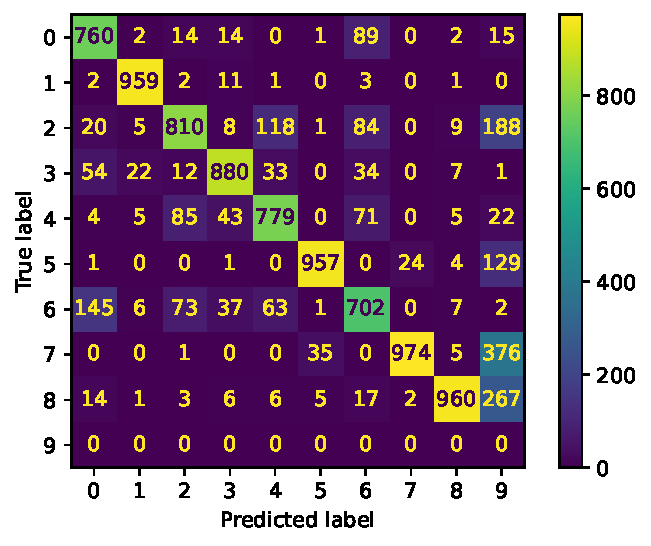
\includegraphics[width=0.35\textwidth]{../Q2/mult_layer_relu/cmat_3.pdf} \\
            2 & 3 \\
            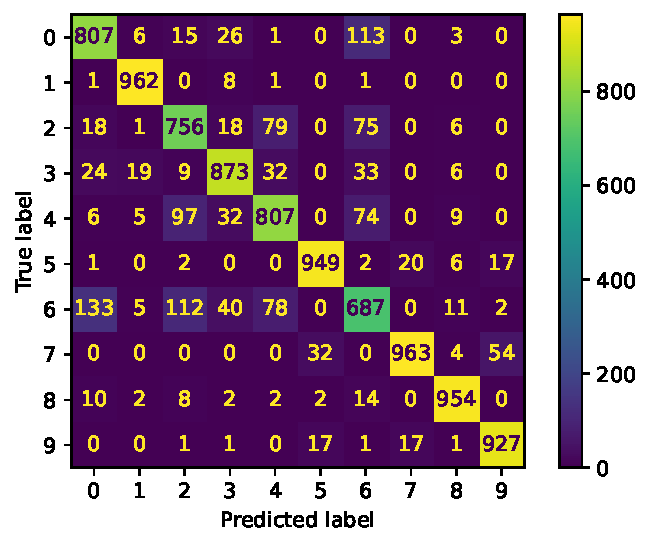
\includegraphics[width=0.35\textwidth]{../Q2/mult_layer_relu/cmat_4.pdf} &
            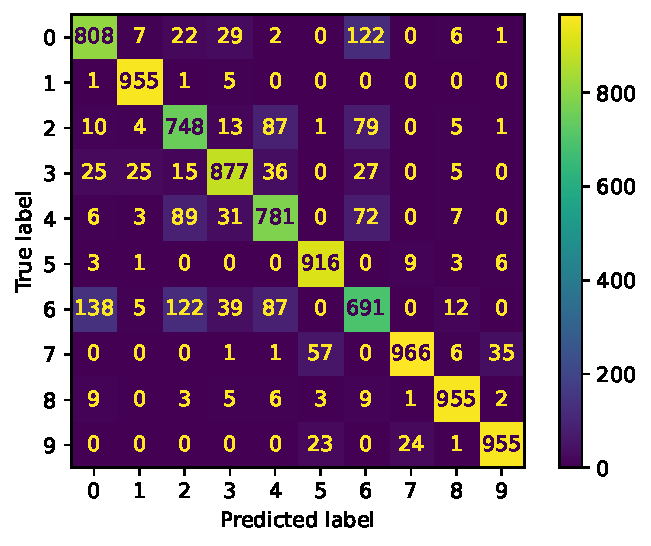
\includegraphics[width=0.35\textwidth]{../Q2/mult_layer_relu/cmat_5.pdf} \\
            4 & 5 
        \end{tabular}
    \end{center}

    The \emph{best} network was found to be a 1x100 network with ReLU activations,
    trained using a constant learning rate. This gave an accuracy of \textbf{88.29 \%}
    on the test dataset and \textbf{93.61 \%} on the train dataset.

    % \begin{center}
    %     \includegraphics[width=0.5\textwidth]{../Q2/best/cmat_best.pdf}
    % \end{center}
    
    \item Cross-Entropy loss for a batch is given by 
    \begin{align*}
        \mathcal{J}^b(\theta) = - \frac 1M \sum_{i=1}^M \sum_{j=1}^{10} 
        y^{(i)}_j\log o^{(i)}_j + (1-y^{(i)}_j)\log (1-o^{(i)}_j)
    \end{align*}

    The derivative of this, with respect to $o$ is 
    \begin{align*}
        \pdv{\mathcal{J}^b(\theta)}{o}\big|_{ij} = - \frac 1M \left( 
        \frac{y^{(i)}_j}{o^{(i)}_j} - \frac{1-y^{(i)}_j}{1-o^{(i)}_j} \right)
    \end{align*}

    After training the best network (1x100) for 397 s using cross-entropy loss, 
    we obtained a training set accuracy of \textbf{95.74 \%} and a test set 
    accuracy of \textbf{87.07 \%}. 

    \item Using the Scikit-Learn MLPClassifier to train a network with the 
    same hyperparameters as the best network we had, we obtain a training set accuracy 
    of \textbf{90.36 \%} and a test set accuracy of \textbf{87.28 \%}. The training
    occurs in 370.87 seconds and takes 200 iterations (the same as our classifier).

    The library implementation does better than the model in 2(f), both of which 
    use Cross Entropy loss as the minimization metric. It also trains slightly 
    faster (27 seconds faster).

\end{enumerate}

\section{Appendix}

The libraries used for this assignment were:
\begin{enumerate}
    \item numpy
    \item pandas
    \item matplotlib
    \item scikit-learn
    \item nltk
    \item scipy
    \item XGBoost
\end{enumerate}

\end{document}
